\documentclass[conference]{IEEEtran}
\IEEEoverridecommandlockouts
\usepackage{cite}
\usepackage{amsmath,amssymb,amsthm}
\usepackage{graphicx}
\usepackage{url}
\def\UrlBreaks{\do\/\do-\do_}
\usepackage{array}
\usepackage{booktabs}
\usepackage{tikz}
\usetikzlibrary{positioning,arrows.meta,fit}
\usepackage[hidelinks]{hyperref}
\newtheorem{proposition}{Proposition}
\newtheorem{remark}{Remark}
\newcommand{\NNodes}{193,191}
\newcommand{\NEdges}{471,240}
\newcommand{\NZones}{7,453}
\newcommand{\NObs}{6,132}
\newcommand{\NFlood}{5,379}
\newcommand{\NWater}{753}
\newcommand{\NOfficial}{1,080}
\newcommand{\NCrowd}{5,052}
\newcommand{\SnapMed}{2.9}
\newcommand{\SnapPninety}{23.6}
\newcommand{\NHazEdges}{14,534}
\newcommand{\NObsEdges}{5,775}
\newcommand{\NPriorEdges}{8,759}
\newcommand{\NConflict}{124}
\newcommand{\CliSec}{3.07}
\newcommand{\NOD}{100}
\newcommand{\WatchCand}{402}
\newcommand{\CzeroEH}{1.61}
\newcommand{\CzeroTW}{0.0113}
\newcommand{\CzeroFF}{1,965.7}
\newcommand{\CzeroHS}{7.8}
\newcommand{\ConeEH}{1.22}
\newcommand{\ConeTW}{0.0078}
\newcommand{\ConeFF}{1,993.0}
\newcommand{\ConeHS}{0.0}
\newcommand{\CthreeEH}{1.52}
\newcommand{\CthreeTW}{0.0100}
\newcommand{\CthreeFF}{1,965.8}
\newcommand{\CthreeHS}{5.3}
\newcommand{\ConeDFF}{27.3}
\newcommand{\ConeDFFlo}{16.9}
\newcommand{\ConeDFFhi}{38.9}
\newcommand{\CthreeDFF}{0.026}
\newcommand{\CthreeDFFlo}{0.003}
\newcommand{\CthreeDFFhi}{0.061}
\newcommand{\ConeDEH}{-0.39}
\newcommand{\ConeDEHlo}{-0.61}
\newcommand{\ConeDEHhi}{-0.21}
\newcommand{\CthreeDEH}{-0.085}
\newcommand{\CthreeDEHlo}{-0.250}
\newcommand{\CthreeDEHhi}{0.002}
\newcommand{\ConeChanged}{30}
\newcommand{\CthreeChanged}{7}
\newcommand{\ShareHRCzero}{30}
\newcommand{\ShareHRCone}{0}
\newcommand{\ShareHRCthree}{29}
\newcommand{\ConeRatio}{1.53}
\newcommand{\ConePninety}{6.2}
\newcommand{\OrigCthreeDetour}{0.27}
\newcommand{\TrueCthreeDetour}{0.0013}
\newcommand{\PbarObsMed}{0.137}
\newcommand{\PbarObsShare}{6.3}
\newcommand{\PbarPriorMed}{0.286}
\newcommand{\ValPaths}{100}
\newcommand{\CalN}{34,256}
\newcommand{\CalPos}{708}
\newcommand{\CthreeBrier}{0.0343}
\newcommand{\CthreeRel}{0.0137}
\newcommand{\CthreeRes}{6.9\times10^{-5}}
\newcommand{\CthreeECE}{0.082}
\newcommand{\CthreeLL}{0.159}
\newcommand{\CthreeAUC}{0.609}
\newcommand{\CtwoBrier}{0.0344}
\newcommand{\CtwoRel}{0.0137}
\newcommand{\CtwoRes}{6.9\times10^{-5}}
\newcommand{\CtwoECE}{0.082}
\newcommand{\CtwoLL}{0.159}
\newcommand{\CtwoAUC}{0.609}
\newcommand{\CfourBrier}{0.0367}
\newcommand{\CfourRel}{0.0161}
\newcommand{\CfourRes}{6.2\times10^{-5}}
\newcommand{\CfourECE}{0.089}
\newcommand{\CfourLL}{0.167}
\newcommand{\CfourAUC}{0.609}
\newcommand{\BetaBrier}{0.2921}
\newcommand{\BetaRel}{0.2712}
\newcommand{\BetaRes}{2.9\times10^{-6}}
\newcommand{\BetaECE}{0.520}
\newcommand{\BetaLL}{0.779}
\newcommand{\BetaAUC}{0.568}
\newcommand{\CalUnc}{0.0202}
\newcommand{\CrowdAUC}{0.566}
\newcommand{\OrigHRzero}{36}
\newcommand{\OrigHRtwo}{72}


\begin{document}
\bstctlcite{IEEEexample:BSTcontrol}

\title{Does Crowd Evidence Help Flood-Aware Routing? An Offline Routing Prototype and a Replay Study on the Chennai Road Network}

\author{\IEEEauthorblockN{Pragatish N}
\IEEEauthorblockA{\textit{\textless Department\textgreater} \\
\textit{Vellore Institute of Technology}\\
Chennai, India \\
\textless E-mail\textgreater}
\and
\IEEEauthorblockN{Ravi \textless Surname\textgreater}
\IEEEauthorblockA{\textit{\textless Department\textgreater} \\
\textit{Vellore Institute of Technology}\\
Chennai, India \\
\textless E-mail\textgreater}
\and
\IEEEauthorblockN{Jyotish \textless Surname\textgreater}
\IEEEauthorblockA{\textit{\textless Department\textgreater} \\
\textit{Vellore Institute of Technology}\\
Chennai, India \\
\textless E-mail\textgreater}}

\maketitle

\begin{abstract}
Navigation apps in Indian cities now display crowd-reported waterlogging, but they do not say how much a report should change a route, how long it should count, or what to do when reports are absent. We built a routing prototype for Chennai that keeps, for each road segment, a flood probability formed from a static susceptibility prior and age-decayed, source-weighted reports; routes on a pessimistic index of that probability; and attaches a structured decision record from which explanations are rendered and checked. We then asked whether the crowd reports, as opposed to the prior, improve routes. On the OpenStreetMap graph of Chennai (193,191 nodes, 471,240 directed edges) with 6,132 geolocated observations from the 2015 floods, all routes were scored under one common reference belief. The default commuter setting changed 7 of 100 routes. Larger risk weights lowered expected hazardous edges per route from 1.61 to 0.98 at a 0.85\% mean detour, but the whole advantage over hard blocking came from prior-only edges; on edges with observations the soft penalty did slightly worse. Against held-out official reports, crowd plus prior routed no better than the prior alone, and adding crowd evidence made the Brier score of the belief worse. We also show that the pessimistic index lowers caution after a single weak report, and we report two implementation faults found in review. The results describe the method on one historical event without depth or negative reports; they do not establish benefit or safety in live use.
\end{abstract}

\begin{IEEEkeywords}
Calibration, crowdsourcing, flood hazards, mobile computing, route planning, uncertainty.
\end{IEEEkeywords}

\section{Introduction}
Pluvial floods cut urban road networks in ways that travel-time routing does not see. Hydrodynamic and network studies show disconnection of intra-urban roads~\cite{yin2016shanghai,zhou2022connectivity}, abrupt network-wide failure from local flooding~\cite{wang2019percolation}, and longer emergency response times~\cite{green2017emergency,coles2017york}; depth--disruption functions relate water depth to safe speed~\cite{pregnolato2017depth}. Chennai flooded severely in 2015 and again in 2023~\cite{vanoldenborgh2016chennai,radhakrishnan2024chennai}, and its built-up area keeps growing~\cite{devi2019sprawl}.

Consumer navigation has started to respond. Google Maps reported that India produced more flood-related alerts on Maps in 2025 than any other country~\cite{ramani2025maps}, and Mappls offers waterlogging and flood-alert report categories~\cite{mappls2026post}. In Chennai, a crowd flood map ran as a pilot from 2017 to 2019~\cite{urbanrisklab2019riskmap}, and a volunteer street-marking effort recorded more than 2,500 flooded streets within a day in 2015~\cite{naik2016flooded}. What these services do not document is how a report should change a route: how much weight a single report deserves, how quickly it should fade, how sparse evidence should be treated, and how the choice should be explained. Crowd reports are also known to be sparse, uneven across neighbourhoods and of varying accuracy~\cite{senaratne2017vgi,esparza2023imbalance,liu2023wazecoverage}.

We built a prototype that makes these choices explicit and then tested whether they matter. The prototype fuses a susceptibility prior with decaying reports in log-odds, routes on a pessimistic index whose strength is set per user class, separates slowdown from harm in the edge cost, and returns a decision record that explanation layers must respect. We ask three questions. RQ1: does the belief-aware cost change routes on a real city graph, and at what travel-time cost? RQ2: do crowd reports add anything to routing or to the belief beyond the static prior? RQ3: does the pessimistic index behave as intended when evidence is sparse?

The contribution is a systems integration and an application case study, not a new algorithm. Every component has precedent, which Section~\ref{sec:related} credits. Specifically, the paper offers:
\begin{itemize}
\item An open design that combines a decaying, source-weighted flood belief, a class-specific pessimistic index, a cost that separates slowdown from harm, and a decision record with a symbolic gate on generated explanations (Sections~\ref{sec:model}--\ref{sec:system}).
\item Two analytical observations: a time-proportional penalty caps an edge's cost at $1+\lambda s$ times free-flow time, and a Wald-type pessimistic index decreases after one report from a source whose reliability is below about 0.63 (Propositions~\ref{prop:cap} and~\ref{prop:dip}).
\item A replay evaluation on the full Chennai graph that scores all configurations under one reference belief, splits exposure into observed and prior-only edges, adds a hybrid baseline, and checks routes against held-out official reports (Sections~\ref{sec:setup}--\ref{sec:results}).
\item An account of what did not work, including two implementation faults that a code review found, so that others building similar systems can avoid them (Section~\ref{sec:lessons}).
\end{itemize}

\section{Related Work}\label{sec:related}
\subsection{Flood impacts and flood-aware routing}
Network studies quantify accessibility loss under floods~\cite{yin2016shanghai,coles2017york,green2017emergency,kasmalkar2020floods,zhou2022connectivity,loreti2022local}, and an Indian study applied a depth--safe-speed curve to estimate how much road length becomes impassable in extreme rainfall~\cite{singh2018vulnerability}. Routing work typically takes the flood state from a model. De~Faria et~al.~\cite{defaria2026routing} drive a time-varying routing optimisation with stormwater-model inundation and flood--speed reductions; Panakkal et~al.~\cite{panakkal2023safer} feed live rainfall into a physical flood model and analyse the resulting network to report road conditions per vehicle class; FLOAT trades travel time against flood risk with tunable weights in evacuation routing~\cite{jao2025float}; and Dijkstra-based, dispatch and reinforcement-learning variants exist~\cite{li2023dijkstra,liang2025rescue,li2025drl,bucar2022route}. Closer to our setting, Panakkal and Padgett combine gauges, social media and imagery with physics models to infer the flood status of individual links~\cite{panakkal2024eyes}; Lupa et~al.~\cite{lupa2026stars} route ambulances on satellite-derived passability and bracket uncertainty with two products; Fu et~al.~\cite{fu2026social} turn social-media events into a spatially decaying impedance field; and Itoi et~al.~\cite{itoi2017offline} built an offline evacuation app that treats a user's departure from the suggested path as evidence of a blocked segment. Flood-aware travel routing also appears in patents~\cite{ibm2013patent,uber2020patent}. We are not aware of a flood router that discounts reports by age and source and lets the amount of evidence change the cost; Section~\ref{sec:results} suggests that, on our data, doing so did not help.

\subsection{Sensing road flooding}
Navigation-app reports can indicate flooded roads~\cite{praharaj2021waze,safaei2023waze,lowrie2022waze}, and road-inundation probability has been predicted from crowd reports and traffic data~\cite{yuan2023predicting}; crowd reports can stand in for some physical sensors~\cite{esparza2024crowd}. Their coverage drifts with traffic volume~\cite{liu2023wazecoverage} and is unequal across neighbourhoods~\cite{esparza2023imbalance}, which motivates explicit under-reporting models~\cite{agostini2024underreport}. Vehicle traces give a second signal: floating-car speed thresholds detect waterlogging~\cite{hu2018fcd}, drops in taxi passing rates map flooded roads~\cite{kong2022taxi}, probe-vehicle presence tracks inundation extent~\cite{hiramoto2025probe}, and a likelihood test on probe activity detects road closures~\cite{pietrobon2019closure}. Low-cost ultrasonic sensors measure street-level depth directly~\cite{mydlarz2024floodnet}. For Chennai, social-media posts have been used to map 2015 inundation depths~\cite{karmegam2021chennai} and hotspots~\cite{sattaru2021utilizing}, and flood susceptibility has been mapped from historical flood locations~\cite{natarajan2021flood}. Our replay corpus contains only positive reports; the traversal-based work above is the most direct route to the negative evidence it lacks.

\subsection{Routing under uncertainty and ambiguity}
Stochastic and reliable shortest paths optimise expected time, variance or on-time arrival~\cite{frank1969probabilistic,sivakumar1994variance,fu1998expected,millerhooks2000least,nie2009ontime,xing2011reliable,samaranayake2012reliable}; chance constraints~\cite{charnes1959chance} and robust optimisation~\cite{bertsimas2003robust} express caution. Hazardous-materials routing minimises catastrophe or worst-case risk measures~\cite{erkut2000catastrophe,toumazis2016wcvar}, and safety-aware navigation trades crash or crime risk against time~\cite{galbrun2016safe,krumm2017riskaware,rohmann2026bayesian}. When blocked roads are discovered en route, the problem becomes the Canadian Traveller Problem~\cite{papadimitriou1991ctp}, for which uncertainty-aware policies beat optimistic ones~\cite{eyerich2010ctp}. Preferring known risk to unknown risk is the classic ambiguity aversion of Ellsberg~\cite{ellsberg1961risk}, formalised as maxmin expected utility~\cite{gilboa1989maxmin}; our index is a crude, per-edge version of that idea. For evidence fusion we follow occupancy-grid log-odds updating~\cite{elfes1989occupancy}; decay of trust with age appears in beta reputation systems~\cite{josang2002beta} and in the persistence filter~\cite{rosen2016persistence}. Landmark (ALT) search~\cite{goldberg2005alt} stays correct when no weight drops below its initial value~\cite{delling2007landmark}.

\subsection{Explaining routes and checking generated text}
Route explanation is a small line of work: inverse optimisation explains why one path beats another~\cite{alsheeb2023explainable}, and minimal sets of congested segments explain why a traffic-aware route differs from the free-flow one~\cite{schild2025route}. A simulator study found that drivers followed recommendations more often when the system explained them~\cite{thill2018adherence}, and a recent position paper warns that conversational navigation can turn a verifiable geometric task into persuasion~\cite{ilyankou2026scenic}. In data-to-text generation, template-then-rewrite pipelines~\cite{kale2020t2g2}, fidelity reranking~\cite{harkous2020datatuner}, entailment-based checking~\cite{dusek2020nli} and error annotation protocols~\cite{thomson2020gold} target the same problem we face; open models still make factual errors on such tasks~\cite{kasner2024quintd}, and neural generation hallucinates in general~\cite{ji2023hallucination}. Small models run on phones~\cite{gemma2025gemma3}, but measured speed and energy vary widely across devices~\cite{xiao2024pockets,laskaridis2024melt}.

\section{Formulation}\label{sec:model}
\subsection{Belief}
Let $G=(V,E)$ be a directed road graph with free-flow time $\tau_0(e)>0$. For edge $e$ and hazard class $c$, a prior log-odds $\ell_0(e)$ encodes susceptibility. Observation $i$ has location $x_i$, time $t_i$, polarity $y_i\in\{+1,-1\}$ and source reliability $\alpha_i\in(0,1)$. With spatial kernel $\kappa$ and class time constant $T_c$,
\begin{align}
\ell(e,t) &= \ell_0(e) + \textstyle\sum_i y_i\,\omega_i(e,t)\,\mathrm{logit}(\alpha_i), \label{eq:fuse}\\
\omega_i(e,t) &= \kappa\big(d(e,x_i)\big)\,e^{-(t-t_i)/T_c}, \nonumber\\
\bar p(e,t) &= \sigma\big(\ell(e,t)\big), \quad n_{\mathrm{eff}}(e,t)=\textstyle\sum_i \omega_i(e,t). \label{eq:neff}
\end{align}
The additive form assumes observations are conditionally independent given the hazard state. The prior is a susceptibility map, so~\eqref{eq:fuse} treats it as the probability of flooding given that an event is under way; the prototype has no event gate, which matters outside an event (Section~\ref{sec:lessons}).

\subsection{Pessimistic index}
The router uses
\begin{equation}
\tilde p(e,t) = \min\Big\{1,\ \bar p + z\sqrt{\bar p(1-\bar p)/(n_{\mathrm{eff}}+1)}\Big\}, \label{eq:pess}
\end{equation}
with $z\ge 0$ set per user class ($z=0$ commuter, $z=1.28$ pedestrian, $z=2$ emergency). We call $\tilde p$ an index rather than a bound: $n_{\mathrm{eff}}$ is a sum of kernel weights, not a sample size, and ignores reliability, so~\eqref{eq:pess} carries no coverage guarantee. For fixed $\bar p$, $\tilde p$ falls as $n_{\mathrm{eff}}$ grows. The intent was that thin evidence should make the router more cautious, and that ageing evidence should not make a road look clear. A common alternative prices an edge as $\tau_0(1+\lambda RC)$ with a confidence $C$ that decays with age, so the penalty vanishes as evidence ages; this is ambiguity-seeking when the correct no-information default is the prior rather than zero. Equation~\eqref{eq:pess} returns to the prior instead. However, $\bar p$ and $n_{\mathrm{eff}}$ move together, and the intent fails along real evidence paths.

\begin{proposition}[Non-monotone response to weak reports]\label{prop:dip}
Let an edge carry no observations, so $\bar p=p_0$ and $n_{\mathrm{eff}}=0$, and add one fresh positive report with $\omega=1$ and reliability $\alpha$. For $z>0$ there is a threshold $\alpha^*(p_0,z)$ such that $\tilde p$ decreases when $\alpha<\alpha^*$. For $p_0\in[0.02,0.10]$, $\alpha^*\approx0.63$ at $z=1.28$ and $\alpha^*\approx0.645$ at $z=2$.
\end{proposition}
\begin{IEEEproof}
The report raises $\bar p$ from $p_0$ to $\sigma(\mathrm{logit}\,p_0+\mathrm{logit}\,\alpha)$ and halves the variance term's denominator. For $\alpha$ near $0.5$ the mean barely moves while the band shrinks by a factor $\sqrt2$, so $\tilde p$ falls; for $\alpha$ near 1 the mean rise dominates. Continuity gives a crossing, which we located numerically by root finding.
\end{IEEEproof}
With $p_0=0.05$ and crowd reliability $0.6$, the index goes from 0.329 with no reports to 0.309 with one report, 0.333 with two and 0.380 with three at $z=1.28$, and from 0.486 to 0.441, 0.461 and 0.509 at $z=2$. Crowd reports make up 82\% of our corpus, so a classwise caution dial that was meant to reward sparse evidence instead penalises the first reports. An ageing report has the same effect at every $z$. A Bayesian alternative avoids this: under a beta posterior one positive observation always raises an upper quantile. The index also saturates: at $z=2$ every prior-only edge with $p_0\ge0.25$ has $\tilde p=1$.

\subsection{Edge cost}
Slowdown and harm enter separately:
\begin{equation}
w_\lambda(e,t)=\tau_0(e)\big[1+\tilde p\,(\delta-1)\big] + \lambda\,\tilde p\,s_c\,\tau_0(e), \label{eq:cost}
\end{equation}
where $\delta=\max\{1, v_0(e)/v_{\mathrm{safe}}(h)\}$ comes from the depth--disruption function of Pregnolato et~al.~\cite{pregnolato2017depth} at depth $h$ ($\delta=1$ when depth is unknown), $s_c$ is class severity and $\lambda\ge0$ the risk weight. An edge is removed when a reported depth exceeds the class threshold $h_{\max}$ and $\tilde p\ge\varepsilon$, a point surrogate for $\Pr[h>h_{\max}]\le\varepsilon$~\cite{charnes1959chance}. Both added terms are non-negative, so $w_\lambda\ge\tau_0$; landmark potentials on $\tau_0$ would therefore stay feasible~\cite{delling2007landmark}, although the prototype does not use them (Section~\ref{sec:system}).

\begin{proposition}[Bounded deterrence]\label{prop:cap}
With $\delta=1$, $w_\lambda/\tau_0=1+\lambda\tilde p s_c\le1+\lambda s_c$. A route avoiding hazardous edges of total free-flow time $T_h$ is chosen only if its extra free-flow time is below $\lambda\sum_e\tilde p_e s_c\tau_0(e)\le\lambda s_cT_h$.
\end{proposition}
\begin{IEEEproof}
Substitute $\delta=1$ in~\eqref{eq:cost}, use $\tilde p\le1$, and compare the summed costs of the two routes.
\end{IEEEproof}
With the commuter setting $\lambda=0.3$, $s_c=1$, a 60~s flooded segment justifies at most an 18~s detour even at $\tilde p=1$, and short, severe segments such as railway underpasses are cheap. No corpus record carries depth, so in all experiments $\delta=1$ and the chance constraint never fires.

\section{System as Implemented}\label{sec:system}
Fig.~\ref{fig:arch} shows the design and Table~\ref{tab:status} what exists. One Dart routing package (compressed-sparse-row graph, bidirectional Dijkstra) is imported by the Flutter client and compiled to a command-line tool for the evaluation harness, so the evaluated and shipped routers share code. A landmark (ALT) module exists and is unit-tested but is not on the query path. The belief package implements~\eqref{eq:fuse}--\eqref{eq:pess} as pure functions and rejects malformed inputs at run time, since a not-a-number value would otherwise let the chance constraint fail open. The client stores observations in SQLite with an R*-tree index~\cite{beckmann1990rstar} and queues local reports in an outbox; the server keeps an append-only, grow-only observation log~\cite{shapiro2011crdt}. Records carry hybrid logical clock stamps~\cite{kulkarni2014hlc}, but synchronisation pages by arrival order, so a report made offline and uploaded late can be skipped by clients that have already synchronised past it.

\begin{figure}[t]
\centering
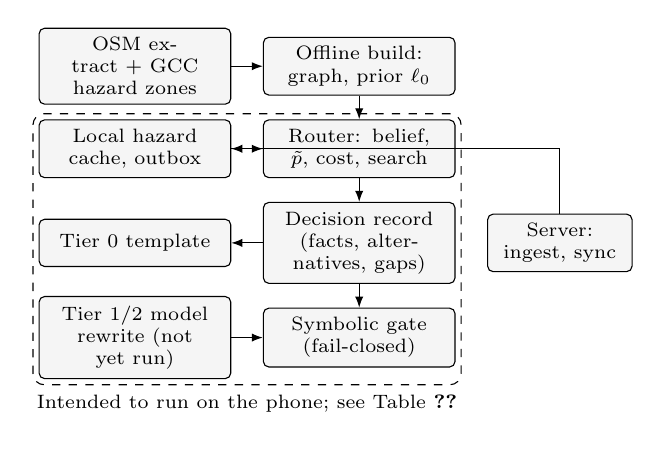
\begin{tikzpicture}[font=\scriptsize, node distance=3mm and 4mm,
  b/.style={draw, rounded corners=2pt, align=center, fill=gray!8, minimum height=6mm, text width=2.2cm},
  a/.style={-{Latex[length=1.4mm]}}]
\node[b] (osm) {OSM extract + GCC hazard zones};
\node[b, right=of osm] (build) {Offline build: graph, prior $\ell_0$};
\node[b, below=of build] (router) {Router: belief, $\tilde p$, cost, search};
\node[b, left=of router] (cache) {Local hazard cache, outbox};
\node[b, below=of router] (trace) {Decision record (facts, alternatives, gaps)};
\node[b, left=of trace] (t0) {Tier 0 template};
\node[b, below=of trace] (ver) {Symbolic gate (fail-closed)};
\node[b, left=of ver] (t12) {Tier 1/2 model rewrite (not yet run)};
\node[b, right=of trace, text width=1.6cm] (srv) {Server: ingest, sync};
\draw[a] (osm) -- (build); \draw[a] (build) -- (router); \draw[a] (cache) -- (router);
\draw[a] (router) -- (trace); \draw[a] (trace) -- (t0); \draw[a] (trace) -- (ver);
\draw[a] (t12) -- (ver); \draw[a] (srv) |- (cache);
\node[draw, dashed, rounded corners, fit=(cache)(router)(trace)(t0)(ver)(t12), inner sep=2pt, label={[font=\scriptsize]below:Intended to run on the phone; see Table~\ref{tab:status}}] {};
\end{tikzpicture}
\caption{Design of the prototype. The dashed box is the intended on-device part; Table~\ref{tab:status} gives what has been implemented and run.}
\label{fig:arch}
\end{figure}

\begin{table}[t]
\centering
\caption{Implementation Status}
\label{tab:status}
\footnotesize
\begin{tabular}{>{\raggedright\arraybackslash}p{2.6cm}>{\raggedright\arraybackslash}p{5.2cm}}
\toprule
Component & Status\\
\midrule
Router, belief, cost & Implemented; replayed on the full city graph; paths reproduced independently\\
Tier 0 template + gate & Implemented; unit and adversarial tests; no user study\\
Tier 1/2 model rewrite & Code written; never executed on a phone or against the cloud model\\
Flutter client & One fixed origin--destination query in a desktop host; no device run; no report screen; no on-device prior\\
Server and sync & Tested in memory; never deployed; ordering issue above\\
\bottomrule
\end{tabular}
\end{table}

Every query returns a decision record with the chosen route (duration, distance, free-flow duration, hazard penalty), rejected alternatives with their penalised edges ($\bar p$, $\tilde p$, $n_{\mathrm{eff}}$, newest-report age), and data gaps. Tier~0 renders it with templates. Tiers~1 and~2 would ask an on-device or cloud model to rewrite it; a rewrite is shown only if it passes the checks in Table~\ref{tab:rules}, otherwise the template text is shown. The checks are symbolic and deliberately simple. They are also incomplete in ways that matter: the numeral check does not bind a number to its subject, the comparative check does not test direction, and the absolute-safety check is a phrase list. In review, the gate accepted ``the bridge is dry now, go ahead on Route B'' for a bridge the router had removed, and accepted a reversed comparison. The Tier~0 template itself said a route ``avoids'' a corridor when the chosen route crossed part of it, and reported a delay that compared penalised cost with plain travel time. We therefore make no claim that displayed explanations are verified.

\begin{table}[t]
\centering
\caption{Explanation Gate Checks and Known Gaps}
\label{tab:rules}
\footnotesize
\begin{tabular}{>{\raggedright\arraybackslash}p{1.45cm}>{\raggedright\arraybackslash}p{3.3cm}>{\raggedright\arraybackslash}p{2.9cm}}
\toprule
Check & Rejects text if \ldots & Known gap\\
\midrule
Numerals & a number matches no record value within tolerance & number not tied to its subject\\
Entities & a capitalised name is absent from the record & fails on Tamil script\\
Comparatives & a comparison has no supporting alternative & direction not checked\\
Data gaps & a claim is attached to a no-data corridor & gaps flagged on low-prior edges only\\
Hedging & confidence is low and no hedge appears & phrase list\\
No safety claim & passability is asserted & phrase list; paraphrases pass\\
\bottomrule
\end{tabular}
\end{table}

\section{Experimental Setup}\label{sec:setup}
\subsection{Data}
\emph{Graph.} A drivable graph of Chennai from OpenStreetMap~\cite{haklay2008osm} with \NNodes{} nodes and \NEdges{} directed edges; free-flow speeds are defaults by road class.
\emph{Prior.} \NZones{} Greater Chennai Corporation flood-hazard polygons were mapped to edges within 600~m, with uncalibrated category defaults from 0.02 to 0.45. No elevation or HAND~\cite{nobre2011hand} layer was used.
\emph{Corpus.} \NObs{} observations from three OpenCity 2015 layers (\NFlood{} flood, \NWater{} waterlogging; \NOfficial{} official, \NCrowd{} crowd) were snapped to the nearest directed edge (median \SnapMed~m). The files carry no dates, so all observations share the stamp 2015-12-02T00:00Z; none has depth; all are positive. Some ``official'' points are designated vulnerable locations rather than dated observations.
\emph{Hazard entries.} \NHazEdges{} edges: \NObsEdges{} with observations and \NPriorEdges{} prior-only edges with $p_0\ge0.25$.

\subsection{Configurations and protocol}
C0 is free-flow routing. C1 removes edges with $\bar p\ge\theta$ ($\theta=0.5$ unless stated). C3 is the method of Section~\ref{sec:model}, swept over $z\in\{0,0.5,1,1.28,2\}$ and $\lambda\in\{0.3,1,2,5,10,20\}$. The hybrid removes edges with $\bar p>0.5$ and adds the C3 penalty with $\lambda=5$, $z=0$. A prior-only variant routes on $\ell_0$ alone. Variants that differ only in decay coincide on a single-timestamp corpus and appear only in the calibration study.

We used the harness's \NOD{} origin--destination pairs (pinned seed). An earlier version of our harness scored each configuration by the worst $\tilde p$ on its own route under its own $z$, and counted penalty seconds as travel time; both make configurations incomparable. Here every route is scored under one reference belief (C3 $\bar p$ at the replay clock), and detours are in free-flow time. Metrics are $\sum_{e\in P}\bar p_e$ (expected hazardous edges per route), split into observed and prior-only edges; the share of routes containing an edge with $\bar p\ge0.5$; and extra free-flow time relative to C0. Paired differences carry 95\% bootstrap intervals (5,000 resamples). C0, C1 and the default C3 routes come from the production router; a SciPy re-implementation of~\eqref{eq:cost} reproduced the production C3 node sequences on \ValPaths{} of \NOD{} pairs and was used for the sweep. Because the reference belief is the model's own, we add one check that does not use it: the mean number of edges carrying an official report on each route, with routing beliefs built from the prior alone or from prior plus crowd reports.

\subsection{Calibration study}
With no confirmed-absent reports, the label is a source holdout: a crowd-reported edge is positive if it also has an official report. Predictors see the prior and crowd reports, with report ages of 0, 1, 6, 24, 72 and 168~h simulated from the single timestamp. The pool has 4,876 crowd edges at six ages (29,256 rows, 708 positives) plus 5,000 randomly sampled edges without reports, labelled negative, for \CalN{} rows. Baselines are a single decay constant (C2), a six-hour time-to-live (C4), a beta reputation model with forgetting~\cite{josang2002beta}, the prior alone and climatology. We report the Brier score with its decomposition~\cite{brier1950verification,murphy1973partition}, the Brier skill score against climatology, and AUROC~\cite{fawcett2006roc}.

\section{Results}\label{sec:results}
\subsection{RQ1: the default barely acts; larger weights trade time for exposure}
The default commuter setting ($z=0$, $\lambda=0.3$) changed \CthreeChanged{} of \NOD{} routes, added \CthreeDFF~s of free-flow time on average (95\% CI [\CthreeDFFlo, \CthreeDFFhi]), and changed expected hazardous edges per route by $\CthreeDEH$ ([$\CthreeDEHlo$, $\CthreeDEHhi$]), an interval that includes zero. \ShareHRCthree\% of its routes still crossed an edge with $\bar p\ge0.5$, against \ShareHRCzero\% for C0 (Table~\ref{tab:sweep}). Proposition~\ref{prop:cap} explains this: at $\lambda=0.3$ a hazardous edge costs at most 1.3 times its free-flow time. Hard blocking changed \ConeChanged{} routes at a \ConeRatio\% mean detour (\ConeDFF~s, [\ConeDFFlo, \ConeDFFhi]) and removed all $\bar p\ge0.5$ crossings by construction. Larger weights lowered exposure steadily (Fig.~\ref{fig:pareto}): at $z=0$, $\lambda=5$ gave 0.98 expected hazardous edges at a 0.85\% mean detour and $\lambda=20$ gave 0.44 at 4.53\%. At matched detour, higher $z$ did not lower reference exposure. This cannot count for or against pessimism, because a belief cannot be shown wrong by scoring against itself.

\begin{table*}[t]
\centering
\caption{Route Exposure Under a Common Reference Belief (C3 $\bar p$ at the Replay Clock), 100 Origin--Destination Pairs}
\label{tab:sweep}
\footnotesize
\begin{tabular}{lrrrrrrr}
\toprule
Config. & $z$ & $\lambda$ & Mean extra & P90 extra & $\sum\bar p$ & Share $\bar p\!\geq\!0.5$ & TW-mean $\bar p$\\
 & & & time (\%) & time (\%) & per route & (\%) & \\
\midrule
C0 (free-flow) & -- & -- & 0.00 & 0.00 & 1.61 & 30 & 0.0113\\
C1 (block $\bar p\geq0.5$) & 0 & 0 & 1.53 & 6.20 & 1.22 & 0 & 0.0078\\
C3 & 0 & 0.3 & 0.00 & 0.00 & 1.52 & 29 & 0.0100\\
C3 & 0 & 5 & 0.85 & 2.73 & 0.98 & 21 & 0.0062\\
C3 & 0 & 20 & 4.53 & 13.93 & 0.44 & 6 & 0.0023\\
C3 & 1 & 5 & 3.06 & 10.51 & 0.66 & 14 & 0.0037\\
C3 & 1 & 20 & 9.53 & 25.57 & 0.26 & 5 & 0.0009\\
C3 & 2 & 0.3 & 0.05 & 0.07 & 1.41 & 28 & 0.0094\\
C3 & 2 & 5 & 4.25 & 12.20 & 0.55 & 11 & 0.0028\\
C3 & 2 & 20 & 12.72 & 30.97 & 0.18 & 4 & 0.0005\\
\bottomrule
\end{tabular}

\end{table*}

\begin{figure}[t]
\centering
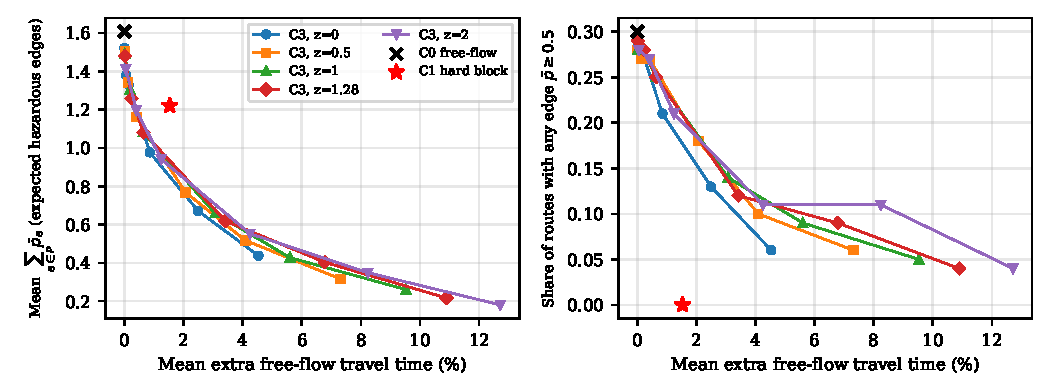
\includegraphics[width=\columnwidth]{fig_pareto_common}
\caption{Exposure against mean extra free-flow time for the C3 sweep ($\lambda$ increases along each line), C0 and C1, all scored under the same reference belief. C1 is zero in the right panel by construction.}
\label{fig:pareto}
\end{figure}

\subsection{RQ2: the gains come from the prior, not the crowd}
Fig.~\ref{fig:decomp} splits exposure by edge type. Relative to C1, C3 with $\lambda=5$ lowered $\sum\bar p$ by 0.24; this difference is $-0.28$ on prior-only edges and $+0.04$ on observed edges. The soft penalty therefore did better than blocking only because a 0.5 threshold cannot see prior-only edges, whose $\bar p$ never exceeds 0.45, and it did slightly worse where reports exist. The hybrid closed most of the gap: 0.79 expected hazardous edges at a 2.14\% detour with no $\bar p\ge0.5$ crossings, near the C3 curve at the same detour. The trade-off between cumulative exposure and worst-segment exposure that we had presented as forced is largely an artefact of omitting this baseline. Lowering the block threshold to 0.25 left 3 of 100 pairs disconnected.

\begin{figure}[t]
\centering
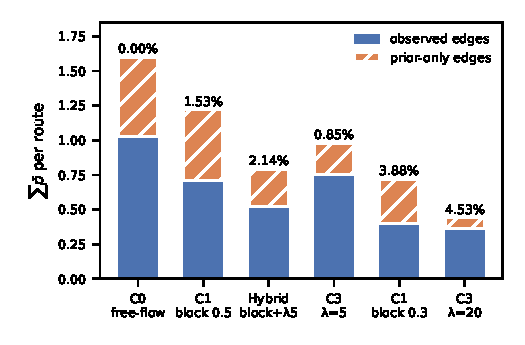
\includegraphics[width=\columnwidth]{fig_decomp}
\caption{Expected hazardous edges per route under the reference belief, split into edges with observations and prior-only edges. Labels give mean extra free-flow time.}
\label{fig:decomp}
\end{figure}

Against held-out official reports (Table~\ref{tab:holdout}), the prior alone and prior plus crowd reports routed equally well, with the crowd version slightly worse and slightly slower at both risk weights. Hard blocking on the fused belief did not change the count relative to C0. The official layers share the label problems noted below, so this is weak evidence; it is, however, the only check in this paper that does not reuse the model's own belief, and it found no gain from crowd evidence.

\begin{table}[t]
\centering
\caption{Routes Against Held-Out Official Reports (100 Pairs)}
\label{tab:holdout}
\footnotesize
\begin{tabular}{lrrr}
\toprule
Routing belief & Official edges & Routes touching & Detour\\
 & per route & one (\%) & (\%)\\
\midrule
C0 free-flow & 1.27 & 48 & 0.00\\
Prior only, $\lambda=5$ & 1.07 & 44 & 0.45\\
Prior + crowd, $\lambda=5$ & 1.09 & 44 & 0.51\\
Prior only, $\lambda=20$ & 0.86 & 39 & 2.96\\
Prior + crowd, $\lambda=20$ & 0.91 & 40 & 3.39\\
\bottomrule
\end{tabular}
\end{table}

\subsection{RQ2 continued: calibration}
Table~\ref{tab:cal} gives the calibration results. Every model scored worse than climatology (Brier 0.0202): the Brier skill score was $-0.70$ for C3 and $-0.81$ for C4. On the crowd pool at age zero, the prior alone scored 0.0361 and C3 0.0478; adding crowd evidence worsened the belief, and the score improved as crowd weight decayed. Resolution was near zero ($\CthreeRes$). The pooled AUROC of \CthreeAUC{} is inflated by the 5,000 report-free negatives; on the crowd pool it was \CrowdAUC, and within the area covered by GCC hazard zones neither the prior (0.456) nor C3 (0.455) discriminated at all, while edge length alone reached 0.651. Class-specific decay (C3) was indistinguishable from a single constant (C2), but with simulated ages this is not a test of decay. The beta baseline has no base rate and predicts at least 0.5 on every reported edge, which explains its score.

\begin{table}[t]
\centering
\caption{Calibration Against the Source-Holdout Label (\CalN{} Rows, \CalPos{} Positives)}
\label{tab:cal}
\footnotesize
\setlength{\tabcolsep}{3pt}
\begin{tabular}{lrrrr}
\toprule
Model & Brier & BSS & Adapt. ECE & AUROC\\
\midrule
Climatology & 0.0202 & 0 & -- & 0.500\\
C3 class-specific decay & \CthreeBrier & $-0.70$ & \CthreeECE & \CthreeAUC\\
C2 single decay & \CtwoBrier & $-0.70$ & \CtwoECE & \CtwoAUC\\
C4 fixed TTL (6 h) & \CfourBrier & $-0.81$ & \CfourECE & \CfourAUC\\
Beta reputation~\cite{josang2002beta} & \BetaBrier & $-13.4$ & \BetaECE & \BetaAUC\\
\bottomrule
\end{tabular}
\end{table}

\begin{figure*}[t]
\centering
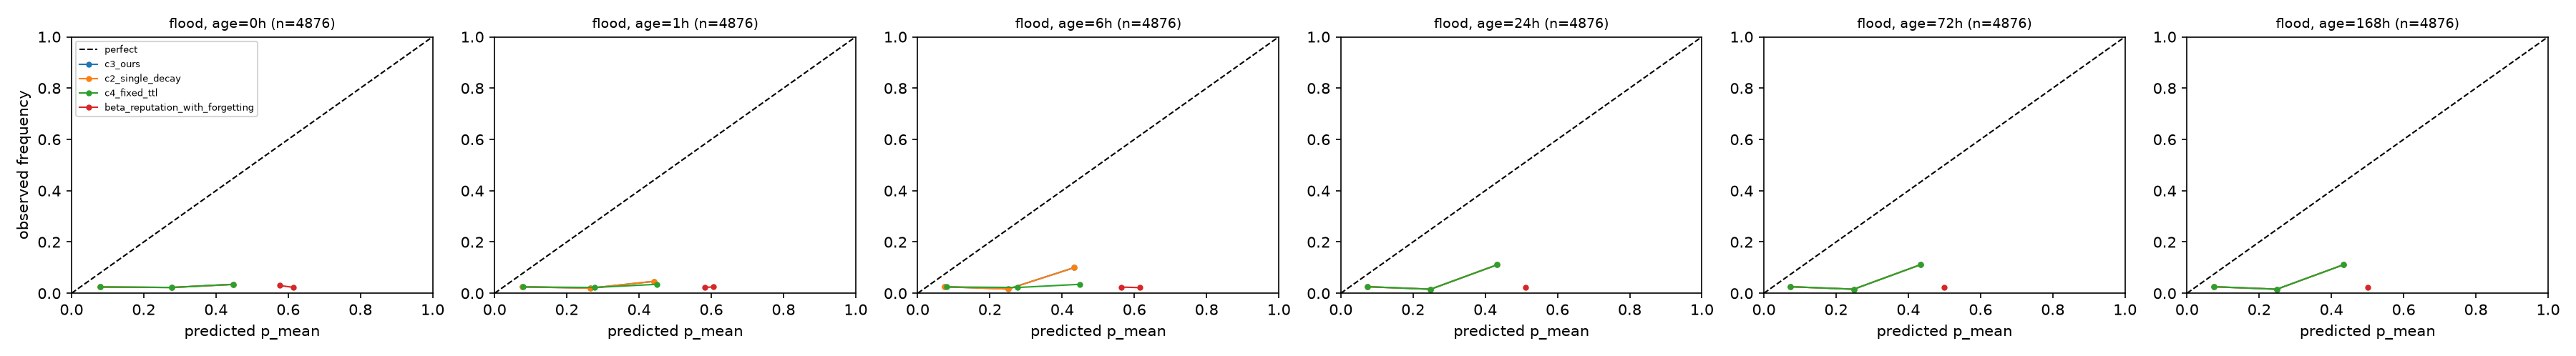
\includegraphics[width=0.85\textwidth]{fig_reliability}
\caption{Reliability diagrams for the flood class by simulated report age (0 to 168 h). All models over-predict relative to the proxy label.}
\label{fig:rel}
\end{figure*}

The reliability diagrams (Fig.~\ref{fig:rel}) show predictions far above observed frequencies. Two features of the label explain part of this. A positive requires an official and a crowd report on the same directed edge, so 899 of 1,017 officially reported edges never enter the pool, and 456 negatives have an official point within 100~m. The label is closer to a test of co-location at edge resolution than of flooding.

\subsection{RQ3 and engineering checks}
Proposition~\ref{prop:dip} holds on the corpus parameters: the crowd reliability of 0.6 sits just below $\alpha^*$, so for $z>0$ the first one or two crowd reports on an edge lower $\tilde p$. At $z=1$, median $\tilde p$ was 0.738 on prior-only edges and 0.383 on observed edges, so the emergency and pedestrian classes were steered most strongly by the uncalibrated prior. Two harness runs produced byte-identical traces. The repository reports about 290 automated tests.

\section{What Did Not Work}\label{sec:lessons}
\emph{One-directional evidence.} Each observation was snapped to a single directed edge. Of the \NObsEdges{} observed edges, 5,177 have a reverse twin, and only 2 of those twins carry evidence, although~\eqref{eq:fuse} would weight the twin identically. A flooded two-way street is thus penalised in one direction only. Every exposure figure above shares this bias; it affects all configurations alike, but the absolute numbers undercount exposure.

\emph{Caution in the wrong place.} The index penalises the first weak reports (Proposition~\ref{prop:dip}), saturates on prior-only edges at $z=2$, and gives no penalty on most of the graph, because 97\% of edges have no hazard entry. The prior is applied whether or not an event is under way.

\emph{Explanations.} The gate passed unsafe sentences and the template produced false ones (Section~\ref{sec:system}). When the template failed its own check, the client showed an error rather than a route.

\emph{Offline claim.} The design is offline-first, but nothing has run on a phone (Table~\ref{tab:status}).

\section{Threats to Validity}\label{sec:threats}
\begin{itemize}
\item \emph{Circular reference.} Exposure is measured under the model's own belief; only the official-report check is external, and its labels are partly susceptibility designations.
\item \emph{Corpus.} One event, one timestamp, no depth, no negative reports, so decay, the chance constraint and false avoidance are untested.
\item \emph{Independence.} Correlated crowd reports of one flood inflate certainty in~\eqref{eq:fuse}.
\item \emph{Defaults.} Prior probabilities and speeds are not fitted; 100 pairs, one city.
\end{itemize}

\section{Conclusion}
We asked whether a router that fuses a flood prior with decaying crowd reports, and becomes more cautious when evidence is thin, routes better on a real city graph. On the 2015 Chennai corpus the answer is no, for three reasons we can name. The default penalty was too weak to change routes, as Proposition~\ref{prop:cap} predicts. Where larger penalties helped, the help came from the static prior; crowd reports added nothing against held-out official reports and worsened calibration. The pessimistic index lowered caution after weak reports. These are results about one historical event with poor labels, not a verdict on crowd evidence in general. The next step is data rather than modelling: a time-stamped corpus with independent passability labels, for example from probe-vehicle traces~\cite{hiramoto2025probe,pietrobon2019closure}, subway barrier states or depth sensors~\cite{mydlarz2024floodnet}, together with a Bayesian upper quantile in place of~\eqref{eq:pess}, bidirectional snapping, an event gate on the prior, and a measured pass rate for model-written explanations on a low-cost phone.

\section*{Acknowledgment}
\textless To be completed by the authors.\textgreater

\bibliographystyle{IEEEtran}
\bibliography{refs,extra}

\end{document}
